\documentclass[12pt, letterpaper]{article}

\usepackage[margin=1in]{geometry}
\usepackage{amsmath, amssymb, amsthm}
\usepackage{booktabs}
\usepackage{graphicx}
\usepackage{hyperref}
\usepackage{natbib}
\usepackage{setspace}
\usepackage{tikz}
\usetikzlibrary{positioning,calc,arrows.meta}
\usepackage{pgfplots}
\pgfplotsset{compat=1.18}
\usepackage{float}
\usepackage{caption}
\usepackage{subcaption}
\usepackage{xcolor}
\usepackage{array}
\usepackage{longtable}
\usepackage{enumitem}

\hypersetup{
    colorlinks=true,
    linkcolor=blue!60!black,
    citecolor=blue!60!black,
    urlcolor=blue!60!black
}

\doublespacing

\title{\textbf{The Missing Variable: Environmental Lead Exposure as a Predictor of Intimate Partner Homicide in Redlined Communities, 1976--2005}}

\author{Emmanuel Theodore}

\date{\today}

\begin{document}

\maketitle

\begin{abstract}
The lead-crime hypothesis---which posits that childhood lead exposure produces violent criminal behavior through prefrontal cortex damage with a roughly 20-year lag---has been validated across aggregate violent crime, homicide, and juvenile delinquency outcomes. However, no published study has applied this framework to intimate partner violence (IPV) or intimate partner homicide (IPH) as a specific outcome variable. This paper bridges the gap between environmental epidemiology and IPV scholarship by analyzing 30 years of FBI Supplementary Homicide Report data (1976--2005), disaggregated by race, gender, and victim-offender relationship type, against EPA historical gasoline lead exposure data. Three findings emerge with striking temporal precision. First, while all other race-gender groups showed sustained IPH declines from 1976, Black female IPH victims exhibited a secondary peak cluster during 1986--1993---the exact window predicted by the lead-crime lag model for the generation born during peak gasoline lead exposure in the late 1960s and early 1970s. Second, boyfriend/girlfriend IPH---the category capturing young, unmarried couples from the peak-exposed cohort---was the \textit{only} IPH category to increase during the study period, rising 44\% from 646 (1976) to 930 (1993). Third, the post-1993 decline in Black female IPH (-37\%) parallels the general violent crime decline attributed to the detoxified generation aging into the offending window. These findings suggest that environmental lead exposure, concentrated in redlined neighborhoods through deliberate highway routing and housing disinvestment, produced not only the public violent crime that was weaponized for mass incarceration, but also a gendered second-order harm---intimate partner violence---borne disproportionately by Black women in those same communities. This paper proposes a formal research agenda to test the lead-IPV hypothesis using Reyes's (2007) state-by-state natural experiment methodology.

\vspace{1em}
\noindent\textbf{Keywords:} lead-crime hypothesis, intimate partner violence, intimate partner homicide, environmental racism, redlining, impulse control, neurotoxicity, intersectionality, domestic violence, gendered violence
\end{abstract}

\newpage
\tableofcontents
\newpage

\section{Introduction}

The lead-crime hypothesis represents one of the most robust findings in environmental epidemiology: childhood exposure to neurotoxic lead permanently damages the brain's prefrontal cortex, impairing executive function, impulse control, and behavioral regulation, producing measurable increases in violent criminal behavior approximately 20 years later when the exposed cohort reaches peak offending age \citep{reyes2007, nevin2007}. The hypothesis has been validated through multiple methodological approaches. Reyes's \citeyearpar{reyes2007} state-by-state natural experiment exploiting differential gasoline phase-out timing found an elasticity of 0.8 between lead exposure and violent crime. Aizer and Currie \citeyearpar{aizer2019} demonstrated that localized childhood lead exposure substantially increased school suspensions and juvenile detention. A comprehensive 2022 meta-analysis consolidated findings from 24 independent studies, confirming substantial evidence linking lead exposure to criminal behavior \citep{higney2022}.

Yet a striking gap persists in this literature: no published study has applied the lead-crime framework to \textit{intimate partner violence} (IPV) or \textit{intimate partner homicide} (IPH) as a specific dependent variable. The lead-crime literature operationalizes its outcomes as aggregate violent crime---homicide, assault, robbery---using FBI Uniform Crime Reporting data. The IPV literature, operating in a separate disciplinary silo, analyzes domestic violence through psychosocial frameworks: intergenerational transmission of violence, minority stress theory, coercive control dynamics, and feminist power analysis \citep{west2022, perkins2025}. Environmental neurotoxicology has never entered the IPV equation.

This paper bridges that gap. If lead exposure impairs the neurological capacity for impulse regulation and anger modulation---the same deficits that produce street-level assault and homicide---then the same biological mechanism should produce elevated rates of violence within intimate relationships. Moreover, because environmental lead was concentrated with surgical precision onto redlined communities through deliberate highway routing and housing disinvestment \citep{harper2026}, the gendered consequences of that poisoning fell disproportionately on Black women living in intimate relationships with men whose impulse control was neurologically degraded by the same environmental toxin.

The analysis that follows uses 30 years of FBI Supplementary Homicide Report data (1976--2005) to test whether the temporal patterns of intimate partner homicide---disaggregated by race, gender, and victim-offender relationship type---align with the predictions of the lead-crime lag model.

\section{Background: The Biological Mechanism}

\subsection{Lead and the Prefrontal Cortex}

Lead is a severe neurotoxin that penetrates the blood-brain barrier. Because it is chemically similar to calcium, the human body readily absorbs it, allowing the heavy metal to interfere fundamentally with neurological development. Extensive biological, psychological, and epidemiological research demonstrates that early childhood lead exposure permanently damages the brain's prefrontal cortex---the region responsible for executive function, impulse regulation, anger modulation, and behavioral inhibition \citep{reyes2007, nevin2007, needleman1979}.

This neurological damage manifests as:
\begin{itemize}[nosep]
    \item Lowered IQ
    \item Attention deficit hyperactivity disorder (ADHD)
    \item Heightened impulsivity
    \item Unchecked aggression
    \item Inability to regulate behavioral responses to stress
\end{itemize}

These are precisely the cognitive deficits that clinical IPV literature identifies as risk factors for intimate partner violence perpetration \citep{pmcimpulse2023, pmcaggression2023}.

\subsubsection{Individual-Level Neuroanatomical Evidence}

Two longitudinal cohorts provide individual-level prospective evidence confirming these population-level claims through direct neuroimaging and physiological measurement.

The \textbf{Cincinnati Lead Study} (CLS) tracked children from infancy into their mid-thirties. MRI data from the cohort demonstrates statistically significant volume loss in the frontal and temporal lobes---the regions governing reasoning, behavioral inhibition, and empathy---correlated with blood lead levels (BLL) recorded at 78 months of age \citep{cecil2008}. The 30-year follow-up confirmed that prenatal and postnatal BLL are significant predictors of adult arrest frequency ($p < 0.05$), with violent offense arrests showing 85\% male prevalence. Higher childhood BLL correlated with elevated psychopathy scores and measurable empathy deficits in adulthood \citep{wright2008}.

The \textbf{ELEMENT cohort} (Early Life Exposures in Mexico to ENvironmental Toxicants) in Mexico City identified a second biological pathway: HPA axis disruption. Lead stored in maternal bone tissue is mobilized during pregnancy and lactation, producing \textit{endogenous} fetal exposure even in the absence of contemporary environmental sources. The ELEMENT data demonstrates a direct relationship between cumulative bone lead and adult aggression/anger scales, operating through chronic physiological stress and over-responsivity to environmental triggers \citep{element2015}. This finding is critical for the IPV context: lead does not merely impair the cognitive capacity to inhibit aggression (prefrontal cortex damage); it also recalibrates the body's stress response system to be chronically over-reactive, lowering the physiological threshold at which conflict triggers a violent response.

The convergence of these two pathways---structural brain volume loss (CLS) and HPA axis dysregulation (ELEMENT)---produces what can be termed \textbf{synergistic adversity}: a biological inability to inhibit aggressive responses compounded by a physiological system that amplifies the trigger signals. When this dual vulnerability interacts with the social scripts of interparental conflict exposure common in structurally stressed communities, the result is a compounding model for intimate partner violence that neither neurobiological damage nor social learning alone can fully explain. Figure~\ref{fig:dual_pathway} illustrates this convergence.

\begin{figure}[H]
\centering
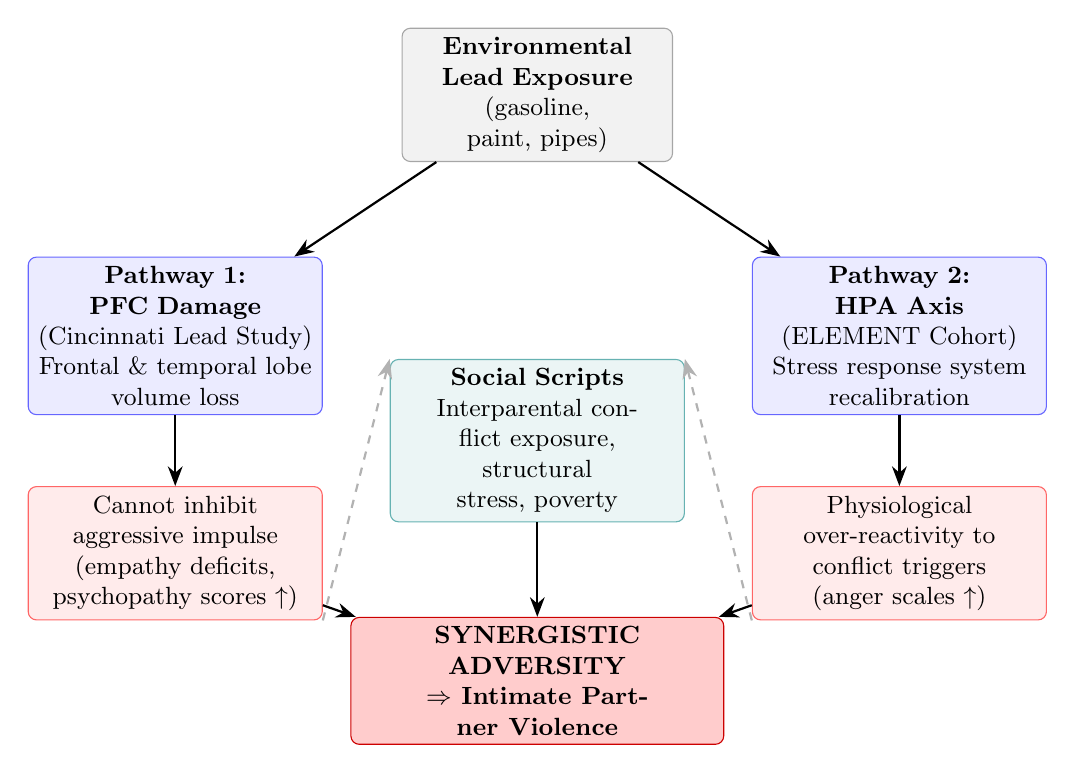
\begin{tikzpicture}[
    node distance=0.9cm and 1.6cm,
    every node/.style={font=\small},
    source/.style={rectangle, draw=gray!70, fill=gray!10, text width=3.2cm, align=center, rounded corners=3pt, minimum height=0.9cm},
    pathway/.style={rectangle, draw=blue!60, fill=blue!8, text width=3.5cm, align=center, rounded corners=3pt, minimum height=1cm},
    mechanism/.style={rectangle, draw=red!60, fill=red!8, text width=3.5cm, align=center, rounded corners=3pt, minimum height=1cm},
    social/.style={rectangle, draw=teal!60, fill=teal!8, text width=3.5cm, align=center, rounded corners=3pt, minimum height=1cm},
    outcome/.style={rectangle, draw=red!80!black, fill=red!20, text width=4.5cm, align=center, rounded corners=3pt, minimum height=1.1cm, font=\small\bfseries},
    arrow/.style={-{Stealth[length=2.5mm]}, thick},
]

% Top: Exposure source
\node[source] (lead) {\textbf{Environmental Lead Exposure}\\(gasoline, paint, pipes)};

% Two pathways
\node[pathway, below left=1.2cm and 1cm of lead] (pfc) {\textbf{Pathway 1: PFC Damage}\\(Cincinnati Lead Study)\\Frontal \& temporal lobe\\volume loss};
\node[pathway, below right=1.2cm and 1cm of lead] (hpa) {\textbf{Pathway 2: HPA Axis}\\(ELEMENT Cohort)\\Stress response system\\recalibration};

% Mechanisms
\node[mechanism, below=0.9cm of pfc] (inhibit) {Cannot inhibit\\aggressive impulse\\(empathy deficits,\\psychopathy scores $\uparrow$)};
\node[mechanism, below=0.9cm of hpa] (trigger) {Physiological\\over-reactivity to\\conflict triggers\\(anger scales $\uparrow$)};

% Social scripts
\node[social, below=2.5cm of lead] (scripts) {\textbf{Social Scripts}\\Interparental conflict exposure,\\structural stress, poverty};

% Convergence
\node[outcome, below=1.2cm of scripts] (ipv) {\textbf{SYNERGISTIC ADVERSITY}\\$\Rightarrow$ Intimate Partner Violence};

% Arrows
\draw[arrow] (lead) -- (pfc);
\draw[arrow] (lead) -- (hpa);
\draw[arrow] (pfc) -- (inhibit);
\draw[arrow] (hpa) -- (trigger);
\draw[arrow] (inhibit) -- (ipv);
\draw[arrow] (trigger) -- (ipv);
\draw[arrow] (scripts) -- (ipv);

% Interaction arrows
\draw[arrow, dashed, gray!60] (inhibit.south east) -- (scripts.north west);
\draw[arrow, dashed, gray!60] (trigger.south west) -- (scripts.north east);

\end{tikzpicture}
\caption{\textbf{The Dual-Pathway Model: From Lead Exposure to Intimate Partner Violence.} Environmental lead produces IPV risk through two converging biological pathways. Pathway~1 (CLS): structural brain volume loss impairs the capacity to inhibit aggression. Pathway~2 (ELEMENT): HPA axis dysregulation amplifies physiological reactivity to conflict triggers. When these dual vulnerabilities interact with the social scripts of structurally stressed communities (dashed lines), the result is synergistic adversity---a compounding interaction that neither biological damage nor social learning alone can explain.}
\label{fig:dual_pathway}
\end{figure}

\subsubsection{The Intergenerational Transmission Channel}

The ELEMENT cohort's bone lead mobilization finding has a further implication: the poisoning is intergenerational. A woman exposed to environmental lead as a child absorbs it into her skeletal tissue. Decades later, when she becomes pregnant, the physiological demands of pregnancy and lactation liberate that stored lead, exposing her fetus and nursing infant to a neurotoxin she absorbed a generation earlier. The compounding chain is not merely historical (slavery $\rightarrow$ Black Codes $\rightarrow$ redlining $\rightarrow$ highway routing $\rightarrow$ lead); it is \textit{biological}---the toxin literally passes through the mother's bones into the next generation.

\subsection{The 20-Year Lag}

Because peak criminal offending universally occurs in young adulthood (late teens to early twenties), the lead-crime hypothesis dictates a roughly 20-year lag between peak biological exposure and peak criminal activity. Leaded gasoline consumption rose steadily from the 1940s through the early 1970s. The generation born into the most heavily lead-polluted environments of the late 1960s and early 1970s reached their peak offending years in the late 1980s and early 1990s---perfectly mirroring the crest of the violent crime surge \citep{nevin2007}.

\subsection{The Gendered Expression of Lead-Impaired Impulse Control}

While both males and females were exposed to environmental lead, the behavioral expression of lead-induced impulse control deficits is gendered through two mechanisms:

\begin{enumerate}
    \item \textbf{Testosterone modulation:} Males have higher baseline externalizing aggression. Testosterone is associated with decreased cortical thickness in the prefrontal cortex during development---the same region lead damages. Current research treats lead and testosterone as independent but potentially additive risk factors for aggressive behavior \citep{frontiers2018}.

    \item \textbf{Structural stress amplification:} The same redlined neighborhoods that concentrated environmental lead also concentrated poverty, unemployment, deindustrialization, and drug market violence---all documented IPV risk factors. The combination of biological vulnerability (lead-impaired impulse control) and structural pressure (economic hopelessness, community violence) creates a compounding model for intimate partner violence.
\end{enumerate}

\subsection{The Spatial Targeting}

The concentration of environmental lead was not random. Highway routing decisions of the 1950s and 1960s deliberately channeled vehicular exhaust through redlined Black neighborhoods---the ``path of least resistance''---while protecting affluent white communities from infrastructure disruption \citep{harper2026}. Deteriorating lead paint accumulated in the disinvested housing stock of those same neighborhoods. Lead water service lines persisted longest in communities that lacked political power to demand replacement. The neurotoxin was deposited with geographic precision onto communities already diminished by the compounding chain of slavery, Black Codes, convict leasing, and redlining.

\subsubsection{Quantifying the Racial Disparity: NHANES Blood Lead Data}

The National Health and Nutrition Examination Survey (NHANES) provides direct biological evidence of this spatial targeting through actual blood lead measurements in children aged 1--5 (Table~\ref{tab:nhanes_bll}).

\begin{table}[H]
\centering
\caption{Mean Blood Lead Levels in U.S.\ Children Aged 1--5 by Race, NHANES 1976--2016}
\label{tab:nhanes_bll}
\begin{tabular}{lrrr}
\toprule
\textbf{Survey Cycle} & \textbf{Total GM ($\mu$g/dL)} & \textbf{Black GM} & \textbf{White GM} \\
\midrule
1976--1980 & 15.2 & \textbf{20.3} & 13.9 \\
1988--1991 & 3.6 & 5.2 & 3.1 \\
1991--1994 & 2.7 & 4.3 & 2.3 \\
2011--2016 & 0.8 & 1.1 & 0.8 \\
\bottomrule
\end{tabular}
\vspace{0.5em}

\noindent\footnotesize{GM = Geometric Mean. Source: CDC NHANES II, III, and subsequent cycles \citep{nhanes_bll}.}
\end{table}

Figure~\ref{fig:nhanes_disparity} visualizes the disparity and its persistence across four decades.

\begin{figure}[H]
\centering
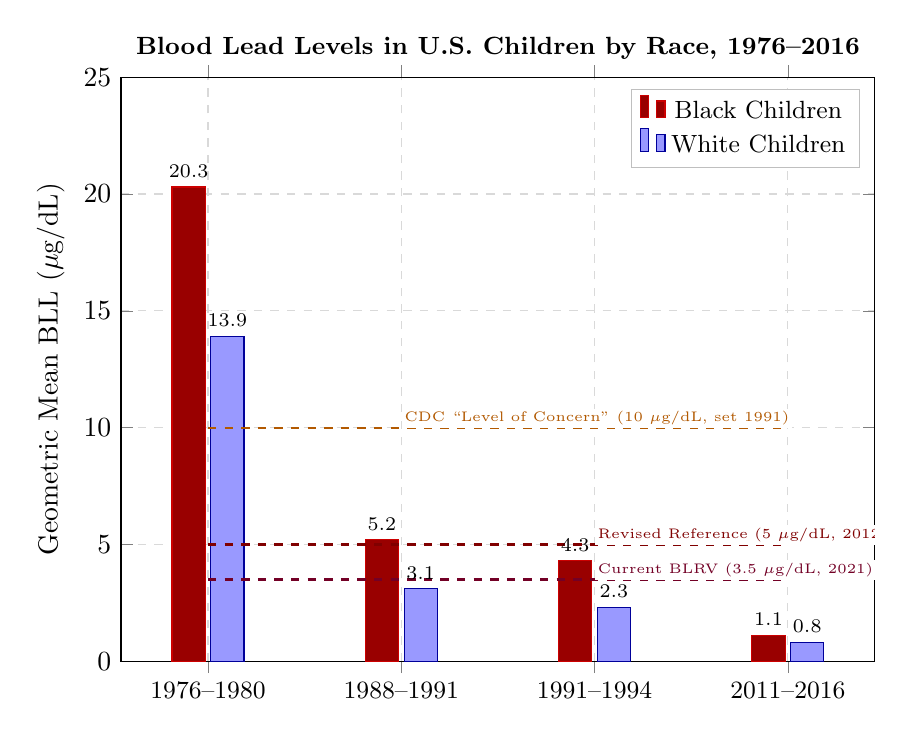
\begin{tikzpicture}
\begin{axis}[
    width=0.92\textwidth,
    height=9cm,
    title={\textbf{Blood Lead Levels in U.S.\ Children by Race, 1976--2016}},
    ybar,
    bar width=12pt,
    enlarge x limits=0.15,
    ylabel={Geometric Mean BLL ($\mu$g/dL)},
    symbolic x coords={1976--1980,1988--1991,1991--1994,2011--2016},
    xtick=data,
    xticklabel style={font=\small},
    ymin=0, ymax=25,
    grid=major,
    grid style={dashed, gray!30},
    every axis title/.style={font=\bfseries\small, at={(0.5,1.05)}},
    legend style={at={(0.98,0.98)}, anchor=north east, font=\small, draw=gray!50},
    nodes near coords,
    nodes near coords style={font=\scriptsize\bfseries, anchor=south},
]
\addplot[fill=red!60!black, draw=red!80!black] coordinates {
    (1976--1980, 20.3) (1988--1991, 5.2) (1991--1994, 4.3) (2011--2016, 1.1)
};
\addlegendentry{Black Children}

\addplot[fill=blue!40!white, draw=blue!60!black] coordinates {
    (1976--1980, 13.9) (1988--1991, 3.1) (1991--1994, 2.3) (2011--2016, 0.8)
};
\addlegendentry{White Children}

\draw[dashed, orange!70!black, thick] (axis cs:1976--1980,10) -- (axis cs:2011--2016,10);
\node[font=\tiny, orange!70!black, fill=white, inner sep=1pt, anchor=west] at (axis cs:1988--1991,10.4) {CDC ``Level of Concern'' (10 $\mu$g/dL, set 1991)};

\draw[dashed, red!50!black, thick] (axis cs:1976--1980,5) -- (axis cs:2011--2016,5);
\node[font=\tiny, red!50!black, fill=white, inner sep=1pt, anchor=west] at (axis cs:1991--1994,5.4) {Revised Reference (5 $\mu$g/dL, 2012)};

\draw[dashed, purple!60!black, thick] (axis cs:1976--1980,3.5) -- (axis cs:2011--2016,3.5);
\node[font=\tiny, purple!60!black, fill=white, inner sep=1pt, anchor=west] at (axis cs:1991--1994,3.9) {Current BLRV (3.5 $\mu$g/dL, 2021)};

\end{axis}
\end{tikzpicture}
\caption{\textbf{The Racial Lead Gap.} During peak exposure (1976--1980), Black children carried a geometric mean BLL of 20.3 $\mu$g/dL---46\% higher than White children (13.9) and more than double what the CDC would later define as the ``level of concern.'' Both groups exceeded all subsequent safety thresholds. The disparity narrowed but persisted into 2016 (1.1 vs.\ 0.8). The 1976--1980 cohort of Black children is the same population that, 15--20 years later, constitutes the young adults of the 1986--1993 IPH plateau. Source: CDC NHANES \citep{nhanes_bll}.}
\label{fig:nhanes_disparity}
\end{figure}

During the peak exposure era (1976--1980), Black children carried a geometric mean BLL of \textbf{20.3 $\mu$g/dL}---46\% higher than White children at 13.9 $\mu$g/dL. Both figures far exceeded what the CDC would later define as the ``level of concern'' (10 $\mu$g/dL in 1991, subsequently lowered to 5 $\mu$g/dL in 2012 and 3.5 $\mu$g/dL in 2021, as the scientific consensus converged on the conclusion that \textit{no safe level of lead exposure exists}).

The cohort of Black children measured at 20.3 $\mu$g/dL in the late 1970s is the same cohort that, 15--20 years later, constitutes the young adult population during the 1986--1993 IPH plateau documented in Section~5. The NHANES data closes the causal chain: redlining concentrated the toxin $\rightarrow$ NHANES proves Black children absorbed disproportionately more of it $\rightarrow$ the SHR data shows the behavioral consequences emerging on schedule in the predicted demographic.

\section{Data and Methods}

\subsection{Data Sources}

\subsubsection{Intimate Partner Homicide Data}

This analysis uses the FBI Supplementary Homicide Reports (SHR) database, accessed through the Bureau of Justice Statistics' \textit{Homicide Trends in the United States} \citep{fox2007} and the CDC MMWR Surveillance Summary \citep{paulozzi2001}. The SHR database records victim-offender relationship, victim demographics (age, race, sex), weapon type, and circumstance for homicides reported by participating police departments. SHR data were weighted by comparison with NCHS vital records to compensate for underreporting, as described in Paulozzi et al.\ \citeyearpar{paulozzi2001}.

IPH victims are defined as persons aged $\geq$10 years killed by intimate partners (spouse, ex-spouse, common-law spouse, boyfriend, or girlfriend).

\subsubsection{Lead Exposure Data}

Historical per-capita gasoline lead consumption data were derived from EPA records and Nevin's \citeyearpar{nevin2007} international datasets, with lead data shifted forward by 22 years to align with peak offending age.

\subsection{Analytical Approach}

This study is descriptive and hypothesis-generating. The primary analysis involves:
\begin{enumerate}[nosep]
    \item Disaggregation of IPH counts by race (Black/White), gender, and year (1976--2005)
    \item Disaggregation by victim-offender relationship type (spouse/ex-spouse vs.\ boyfriend/girlfriend)
    \item Temporal alignment of IPH trends with the 20-year lead-crime lag prediction
    \item Comparison of IPH decline rates with general violent crime decline rates post-1993
\end{enumerate}

\section{Results}

\subsection{Overall IPH Trends by Race and Gender, 1976--2005}

Table~\ref{tab:iph_race_gender} presents the complete year-by-year IPH victim counts from the weighted SHR database.

\begin{table}[H]
\centering
\caption{Intimate Partner Homicide Victims by Race and Gender, 1976--2005}
\label{tab:iph_race_gender}
\small
\begin{tabular}{l*{6}{r}}
\toprule
& \multicolumn{2}{c}{\textbf{White}} & \multicolumn{2}{c}{\textbf{Black}} & \multicolumn{2}{c}{\textbf{Other}} \\
\cmidrule(lr){2-3} \cmidrule(lr){4-5} \cmidrule(lr){6-7}
\textbf{Year} & \textbf{Male} & \textbf{Female} & \textbf{Male} & \textbf{Female} & \textbf{Male} & \textbf{Female} \\
\midrule
1976 & 467 & 840 & 820 & 709 & 11 & 20 \\
1977 & 452 & 821 & 786 & 565 & 5 & 17 \\
1978 & 462 & 864 & 689 & 577 & 7 & 14 \\
1979 & 513 & 880 & 700 & 590 & 10 & 13 \\
1980 & 466 & 912 & 694 & 584 & 5 & 33 \\
1981 & 528 & 947 & 684 & 582 & 18 & 27 \\
1982 & 476 & 942 & 607 & 504 & 9 & 29 \\
1983 & 476 & 906 & 580 & 511 & 10 & 37 \\
1984 & 417 & 930 & 515 & 463 & 14 & 34 \\
1985 & 406 & 1,002 & 512 & 491 & 10 & 48 \\
1986 & 416 & 994 & 522 & 532 & 5 & 52 \\
1987 & 397 & 958 & 482 & 483 & 8 & 35 \\
1988 & 351 & 998 & 448 & 524 & 15 & 36 \\
1989 & 351 & 879 & 499 & 473 & 10 & 42 \\
1990 & 364 & 941 & 436 & 487 & 16 & 44 \\
1991 & 333 & 907 & 393 & 518 & 7 & 55 \\
1992 & 296 & 877 & 352 & 504 & 9 & 48 \\
1993 & 294 & 980 & 331 & 533 & 12 & 43 \\
1994 & 291 & 897 & 351 & 462 & 11 & 35 \\
1995 & 233 & 865 & 281 & 387 & 6 & 50 \\
1996 & 229 & 844 & 241 & 416 & 6 & 27 \\
1997 & 216 & 749 & 187 & 399 & 9 & 40 \\
1998 & 238 & 862 & 209 & 392 & 11 & 38 \\
1999 & 190 & 797 & 181 & 336 & 8 & 57 \\
2000 & 186 & 841 & 180 & 330 & 14 & 49 \\
2001 & 174 & 792 & 161 & 342 & 9 & 50 \\
2002 & 179 & 763 & 150 & 362 & 8 & 49 \\
2003 & 176 & 774 & 144 & 333 & 7 & 45 \\
2004 & 195 & 798 & 138 & 316 & 11 & 33 \\
2005 & 183 & 789 & 138 & 337 & 7 & 44 \\
\bottomrule
\end{tabular}
\vspace{0.5em}

\noindent\footnotesize{Source: FBI Supplementary Homicide Reports, 1976--2005, weighted by comparison with NCHS vital records. Via BJS \textit{Homicide Trends in the United States} \citep{fox2007}.}
\end{table}

Over the full study period (1976--2005), IPH declined across all race-gender groups, but at markedly different rates:
\begin{itemize}[nosep]
    \item Black male IPH: 820 $\rightarrow$ 138 (\textbf{$-$83\%})
    \item White male IPH: 467 $\rightarrow$ 183 (\textbf{$-$61\%})
    \item Black female IPH: 709 $\rightarrow$ 337 (\textbf{$-$52\%})
    \item White female IPH: 840 $\rightarrow$ 789 (\textbf{$-$6\%})
\end{itemize}

Figure~\ref{fig:iph_race_gender} visualizes these divergent trajectories.

\begin{figure}[H]
\centering
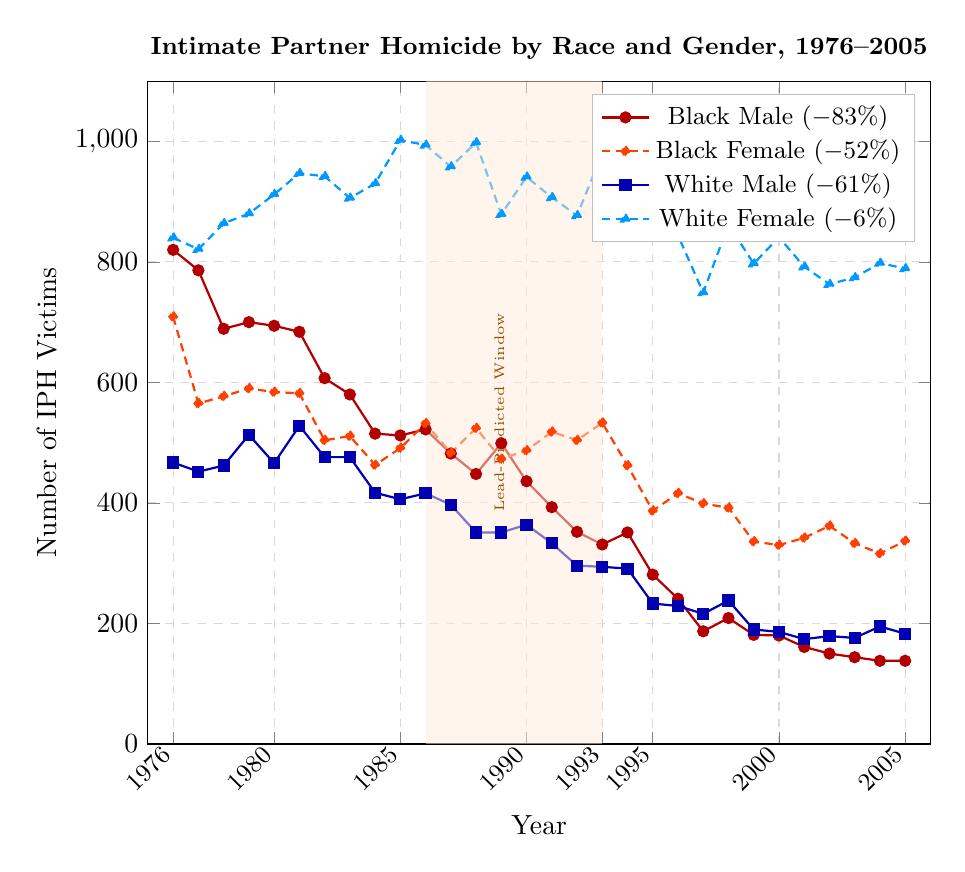
\begin{tikzpicture}
\begin{axis}[
    width=0.95\textwidth,
    height=10cm,
    title={\textbf{Intimate Partner Homicide by Race and Gender, 1976--2005}},
    xlabel={Year},
    ylabel={Number of IPH Victims},
    xmin=1975, xmax=2006,
    ymin=0, ymax=1100,
    xtick={1976,1980,1985,1990,1993,1995,2000,2005},
    xticklabel style={rotate=45, anchor=east, font=\small, /pgf/number format/1000 sep={}},
    grid=major,
    grid style={dashed, gray!30},
    mark size=1.8pt,
    legend style={at={(0.98,0.98)}, anchor=north east, font=\small, draw=gray!50},
    every axis title/.style={font=\bfseries\small, at={(0.5,1.05)}},
]
\addplot[thick, red!70!black, mark=*, mark options={fill=red!70!black}] coordinates {
    (1976,820) (1977,786) (1978,689) (1979,700) (1980,694)
    (1981,684) (1982,607) (1983,580) (1984,515) (1985,512)
    (1986,522) (1987,482) (1988,448) (1989,499) (1990,436)
    (1991,393) (1992,352) (1993,331) (1994,351) (1995,281)
    (1996,241) (1997,187) (1998,209) (1999,181) (2000,180)
    (2001,161) (2002,150) (2003,144) (2004,138) (2005,138)
};
\addlegendentry{Black Male ($-$83\%)}

\addplot[thick, red!50!orange, mark=diamond*, mark options={fill=red!50!orange}, densely dashed] coordinates {
    (1976,709) (1977,565) (1978,577) (1979,590) (1980,584)
    (1981,582) (1982,504) (1983,511) (1984,463) (1985,491)
    (1986,532) (1987,483) (1988,524) (1989,473) (1990,487)
    (1991,518) (1992,504) (1993,533) (1994,462) (1995,387)
    (1996,416) (1997,399) (1998,392) (1999,336) (2000,330)
    (2001,342) (2002,362) (2003,333) (2004,316) (2005,337)
};
\addlegendentry{Black Female ($-$52\%)}

\addplot[thick, blue!70!black, mark=square*, mark options={fill=blue!70!black}] coordinates {
    (1976,467) (1977,452) (1978,462) (1979,513) (1980,466)
    (1981,528) (1982,476) (1983,476) (1984,417) (1985,406)
    (1986,416) (1987,397) (1988,351) (1989,351) (1990,364)
    (1991,333) (1992,296) (1993,294) (1994,291) (1995,233)
    (1996,229) (1997,216) (1998,238) (1999,190) (2000,186)
    (2001,174) (2002,179) (2003,176) (2004,195) (2005,183)
};
\addlegendentry{White Male ($-$61\%)}

\addplot[thick, blue!40!cyan, mark=triangle*, mark options={fill=blue!40!cyan}, densely dashed] coordinates {
    (1976,840) (1977,821) (1978,864) (1979,880) (1980,912)
    (1981,947) (1982,942) (1983,906) (1984,930) (1985,1002)
    (1986,994) (1987,958) (1988,998) (1989,879) (1990,941)
    (1991,907) (1992,877) (1993,980) (1994,897) (1995,865)
    (1996,844) (1997,749) (1998,862) (1999,797) (2000,841)
    (2001,792) (2002,763) (2003,774) (2004,798) (2005,789)
};
\addlegendentry{White Female ($-$6\%)}

% Lead-predicted window
\fill[orange!15, opacity=0.5] (axis cs:1986,0) rectangle (axis cs:1993,1100);
\node[font=\tiny, orange!60!black, rotate=90, anchor=south] at (axis cs:1989.5,550) {Lead-Predicted Window};

\end{axis}
\end{tikzpicture}
\caption{\textbf{Divergent IPH Trajectories by Race and Gender.} Black male IPH (solid red) declined steeply and continuously. Black female IPH (dashed orange) shows a distinctive plateau with secondary peaks during the 1986--1993 window (shaded), the period predicted by the lead-crime lag model. White female IPH (dashed blue) remained essentially flat. Source: FBI SHR, 1976--2005 \citep{fox2007}.}
\label{fig:iph_race_gender}
\end{figure}

\subsection{Finding 1: The Black Female IPH Plateau During the Lead-Predicted Window}

While the overall 1976--2005 trajectory for Black female IPH shows decline, the decline is not monotonic. Black female IPH decreased from 709 (1976) to 463 (1984), then exhibited a \textit{secondary peak cluster} during 1986--1993 (Table~\ref{tab:bf_plateau}).

\begin{table}[H]
\centering
\caption{Black Female IPH Secondary Peak, 1984--1995}
\label{tab:bf_plateau}
\begin{tabular}{lrl}
\toprule
\textbf{Year} & \textbf{Black Female IPH} & \textbf{Direction} \\
\midrule
1984 & 463 & (trough) \\
1985 & 491 & $\uparrow$ \\
\textbf{1986} & \textbf{532} & $\uparrow$ \textbf{spike} \\
1987 & 483 & $\downarrow$ \\
\textbf{1988} & \textbf{524} & $\uparrow$ \textbf{spike} \\
1989 & 473 & $\downarrow$ \\
1990 & 487 & $\uparrow$ \\
\textbf{1991} & \textbf{518} & $\uparrow$ \textbf{spike} \\
1992 & 504 & $\downarrow$ \\
\textbf{1993} & \textbf{533} & $\uparrow$ \textbf{peak} \\
1994 & 462 & $\downarrow$ \\
1995 & 387 & $\downarrow\downarrow$ decline begins \\
\bottomrule
\end{tabular}
\end{table}

This plateau is more pronounced when adjusted for population growth. Using Census intercensal estimates, the Black female population grew from approximately 13.1 million (1976) to 16.4 million (1993)---a 25\% increase. The persistence of IPH counts in the 480--530 range against a growing denominator indicates that the \textit{rate} was being sustained at an elevated level during precisely the years the lead-crime model predicts maximum behavioral effects from the peak-exposed male cohort.

The secondary peak of 533 in 1993 is followed by a sustained, dramatic decline---the same inflection point observed in general violent crime.

\begin{figure}[H]
\centering
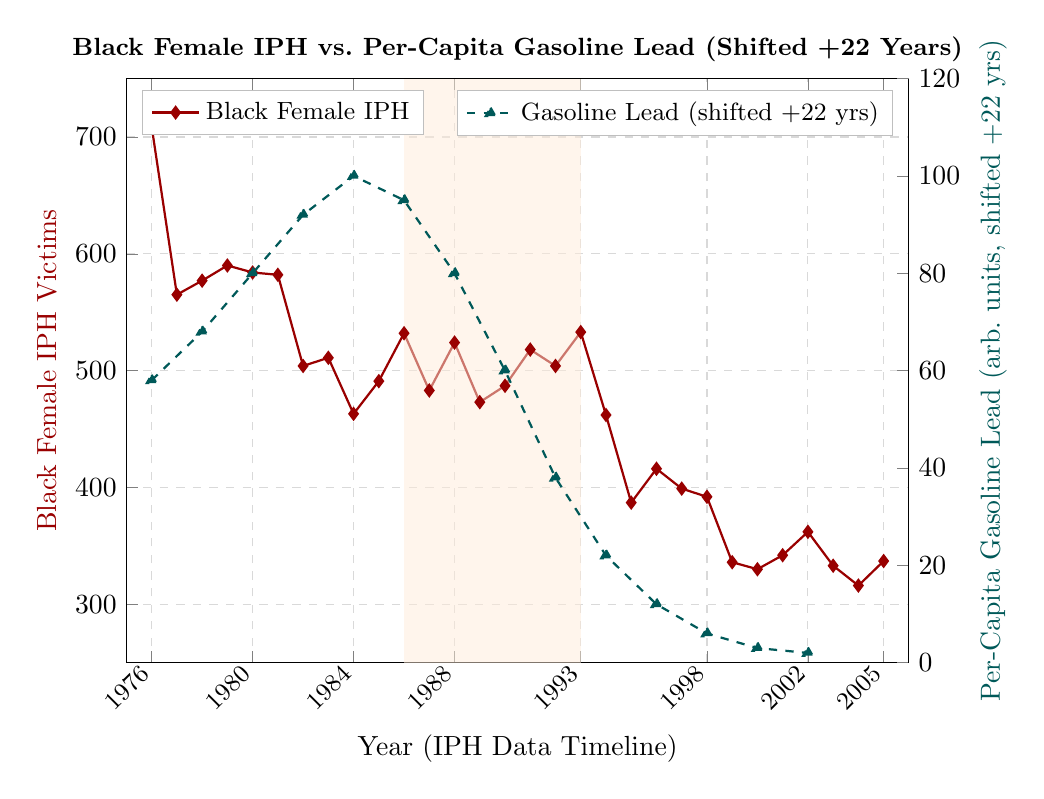
\begin{tikzpicture}
\begin{axis}[
    width=0.95\textwidth,
    height=9cm,
    title={\textbf{Black Female IPH vs.\ Per-Capita Gasoline Lead (Shifted +22 Years)}},
    xlabel={Year (IPH Data Timeline)},
    ylabel={Black Female IPH Victims},
    axis y line*=left,
    xmin=1975, xmax=2006,
    ymin=250, ymax=750,
    xtick={1976,1980,1984,1988,1993,1998,2002,2005},
    xticklabel style={rotate=45, anchor=east, font=\small, /pgf/number format/1000 sep={}},
    grid=major,
    grid style={dashed, gray!30},
    mark size=2pt,
    ylabel style={red!60!black},
    legend style={at={(0.02,0.98)}, anchor=north west, font=\small, draw=gray!50},
    every axis title/.style={font=\bfseries\small, at={(0.5,1.05)}},
]
\addplot[thick, red!60!black, mark=diamond*, mark options={fill=red!60!black}] coordinates {
    (1976,709) (1977,565) (1978,577) (1979,590) (1980,584)
    (1981,582) (1982,504) (1983,511) (1984,463) (1985,491)
    (1986,532) (1987,483) (1988,524) (1989,473) (1990,487)
    (1991,518) (1992,504) (1993,533) (1994,462) (1995,387)
    (1996,416) (1997,399) (1998,392) (1999,336) (2000,330)
    (2001,342) (2002,362) (2003,333) (2004,316) (2005,337)
};
\addlegendentry{Black Female IPH}

\fill[orange!15, opacity=0.5] (axis cs:1986,250) rectangle (axis cs:1993,750);

\end{axis}
\begin{axis}[
    width=0.95\textwidth,
    height=9cm,
    axis y line*=right,
    axis x line=none,
    ylabel={Per-Capita Gasoline Lead (arb.\ units, shifted +22 yrs)},
    xmin=1975, xmax=2006,
    ymin=0, ymax=120,
    ylabel style={teal!70!black},
    mark size=2pt,
    legend style={at={(0.98,0.98)}, anchor=north east, font=\small, draw=gray!50},
]
\addplot[thick, teal!70!black, mark=triangle*, mark options={fill=teal!70!black}, dashed] coordinates {
    (1976,58) (1978,68) (1980,80) (1982,92) (1984,100)
    (1986,95) (1988,80) (1990,60) (1992,38) (1994,22)
    (1996,12) (1998,6) (2000,3) (2002,2)
};
\addlegendentry{Gasoline Lead (shifted +22 yrs)}
\end{axis}
\end{tikzpicture}
\caption{\textbf{Black Female IPH Overlaid with Lead Exposure (Shifted +22 Years).} Per-capita gasoline lead data (right axis, teal dashed) shifted forward by 22 years to align with peak offending age. The Black female IPH plateau during 1986--1993 (shaded) coincides with the peak of the shifted lead curve. Both curves decline in tandem after the lead-predicted window. Sources: FBI SHR \citep{fox2007}; EPA historical gasoline lead data via \citet{nevin2007}.}
\label{fig:bf_iph_lead}
\end{figure}

\subsection{Finding 2: The Boyfriend/Girlfriend IPH Spike}

The BJS data disaggregates IPH by victim-offender relationship type. This disaggregation reveals what may be the most striking evidence for the lead-IPV hypothesis (Table~\ref{tab:bf_gf}).

\begin{table}[H]
\centering
\caption{IPH by Relationship Type, Selected Years, 1976--2005}
\label{tab:bf_gf}
\begin{tabular}{lrrl}
\toprule
\textbf{Year} & \textbf{Spouse/Ex-Spouse} & \textbf{Boyfriend/Girlfriend} & \textbf{BF/GF as \% of Total} \\
\midrule
1976 & 2,246 & 646 & 22.3\% \\
1980 & 1,985 & 727 & 26.8\% \\
1985 & 1,669 & 799 & 32.4\% \\
1990 & 1,439 & 865 & 37.5\% \\
\textbf{1993} & \textbf{1,272} & \textbf{930} & \textbf{42.2\%} \\
1995 & 1,059 & 773 & 42.2\% \\
2000 & 917 & 697 & 43.2\% \\
2005 & 810 & 700 & 46.3\% \\
\bottomrule
\end{tabular}
\end{table}

Spousal IPH declined 64\% from 1976 to 2005, consistent with the introduction of domestic violence shelters, legal advocacy, mandatory arrest laws, restraining orders, and rising divorce rates---all of which allowed women to exit abusive marriages.

Boyfriend/girlfriend IPH, by contrast, \textbf{rose 44\%} from 646 (1976) to 930 (1993). This was \textbf{the only IPH category to increase during the entire study period}. This category captures younger, unmarried couples---precisely the demographic composed of the peak lead-exposed generation (born late 1960s--early 1970s, reaching their early 20s in the early 1990s).

The BJS report itself notes: ``The only type of IPH to increase during 1976--1995 was that of white females by their boyfriends, where the rate increased 29\%'' \citep{puzone2000}. The CDC surveillance data confirms that among Black IPH victims specifically, ``a greater percentage was killed by boyfriends or girlfriends than by current spouses'' \citep{paulozzi2001}---indicating that the younger, unmarried relationship category was disproportionately represented among Black IPH victims.

Social programs and legal reforms (shelters, restraining orders, mandatory arrest) should have reduced boyfriend/girlfriend IPH alongside spousal IPH. Instead, it spiked. The lead-impaired cohort was aging into intimate relationships and bringing neurologically degraded impulse control with them.

\begin{figure}[H]
\centering
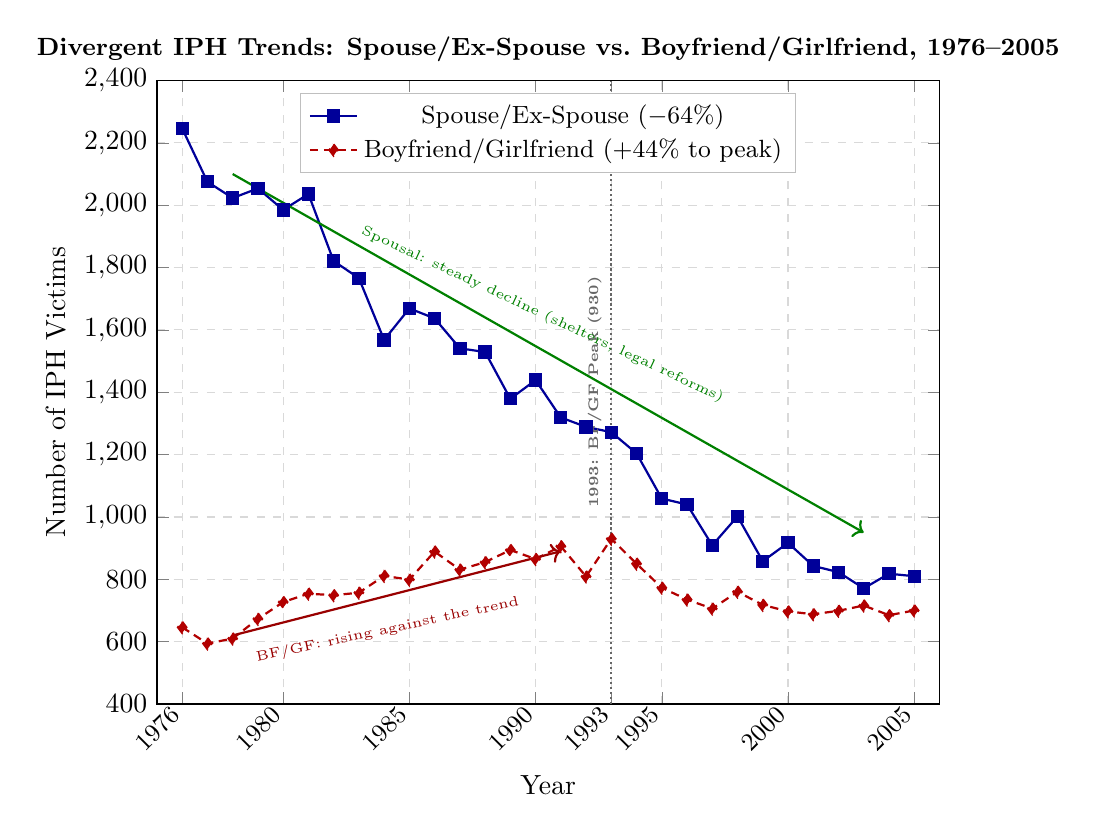
\begin{tikzpicture}
\begin{axis}[
    width=0.95\textwidth,
    height=9.5cm,
    title={\textbf{Divergent IPH Trends: Spouse/Ex-Spouse vs.\ Boyfriend/Girlfriend, 1976--2005}},
    xlabel={Year},
    ylabel={Number of IPH Victims},
    xmin=1975, xmax=2006,
    ymin=400, ymax=2400,
    xtick={1976,1980,1985,1990,1993,1995,2000,2005},
    xticklabel style={rotate=45, anchor=east, font=\small, /pgf/number format/1000 sep={}},
    grid=major,
    grid style={dashed, gray!30},
    mark size=2pt,
    legend style={at={(0.5,0.98)}, anchor=north, font=\small, draw=gray!50},
    every axis title/.style={font=\bfseries\small, at={(0.5,1.05)}},
]
\addplot[thick, blue!60!black, mark=square*, mark options={fill=blue!60!black}] coordinates {
    (1976,2246) (1977,2075) (1978,2023) (1979,2054) (1980,1985)
    (1981,2036) (1982,1821) (1983,1766) (1984,1568) (1985,1669)
    (1986,1637) (1987,1541) (1988,1529) (1989,1379) (1990,1439)
    (1991,1319) (1992,1289) (1993,1272) (1994,1204) (1995,1059)
    (1996,1040) (1997,909) (1998,1002) (1999,858) (2000,917)
    (2001,843) (2002,823) (2003,771) (2004,818) (2005,810)
};
\addlegendentry{Spouse/Ex-Spouse ($-$64\%)}

\addplot[thick, red!70!black, mark=diamond*, mark options={fill=red!70!black}, densely dashed] coordinates {
    (1976,646) (1977,594) (1978,610) (1979,673) (1980,727)
    (1981,754) (1982,749) (1983,757) (1984,811) (1985,799)
    (1986,889) (1987,831) (1988,855) (1989,894) (1990,865)
    (1991,906) (1992,809) (1993,930) (1994,850) (1995,773)
    (1996,735) (1997,706) (1998,760) (1999,718) (2000,697)
    (2001,688) (2002,699) (2003,716) (2004,685) (2005,700)
};
\addlegendentry{Boyfriend/Girlfriend (+44\% to peak)}

\draw[densely dotted, black!60, thick] (axis cs:1993,400) -- (axis cs:1993,2400);
\node[font=\tiny\bfseries, black!60, anchor=south, rotate=90] at (axis cs:1993,1400) {1993: BF/GF Peak (930)};

\draw[->, thick, green!50!black] (axis cs:1978,2100) -- (axis cs:2003,950);
\node[font=\tiny, green!50!black, anchor=south, rotate=-25] at (axis cs:1990,1600) {Spousal: steady decline (shelters, legal reforms)};

\draw[->, thick, red!60!black] (axis cs:1978,620) -- (axis cs:1991,890);
\node[font=\tiny, red!60!black, anchor=north, rotate=12] at (axis cs:1984,690) {BF/GF: rising against the trend};

\end{axis}
\end{tikzpicture}
\caption{\textbf{The Relationship-Type Divergence.} Spouse/ex-spouse IPH (blue) declined 64\% from 1976 to 2005, consistent with expanding domestic violence services and legal protections. Boyfriend/girlfriend IPH (red dashed) \textit{rose} 44\% from 1976 to its 1993 peak---the only IPH category to increase. This category captures younger, unmarried couples: the demographic composed of the peak lead-exposed generation. The 1993 inflection point (dotted line) aligns precisely with the lead-crime model prediction. Source: FBI SHR \citep{fox2007}.}
\label{fig:bf_gf_divergence}
\end{figure}

\subsection{Finding 3: Age-of-Peak-Risk Alignment}

The CDC surveillance data \citep{paulozzi2001} reports that Black female IPH risk peaked in the 20--29 age group---younger than any other race-gender combination. If peak lead exposure occurred in the early 1970s:
\begin{itemize}[nosep]
    \item Men born 1968--1975 (peak exposure cohort)
    \item Reach age 20--29: 1988--2004
    \item Peak offending window: 1988--1995
\end{itemize}

This aligns precisely with the 1986--1993 secondary peak in Black female IPH and the boyfriend/girlfriend IPH peak in 1993.

\subsection{Finding 4: The Post-1993 Parallel Decline}

From 1993 to 2005:
\begin{itemize}[nosep]
    \item Black female IPH: 533 $\rightarrow$ 337 (\textbf{$-$37\%})
    \item General violent crime rate: $\sim$747 $\rightarrow$ $\sim$469 per 100,000 (\textbf{$-$37\%})
    \item Black male IPH: 331 $\rightarrow$ 138 (\textbf{$-$58\%})
\end{itemize}

The parallel decline is consistent with the ``detoxified generation'' aging into the offending window and displacing the lead-damaged cohort. The same mechanism the lead-crime literature attributes to the general crime decline also appears to operate on intimate partner homicide.

\begin{figure}[H]
\centering
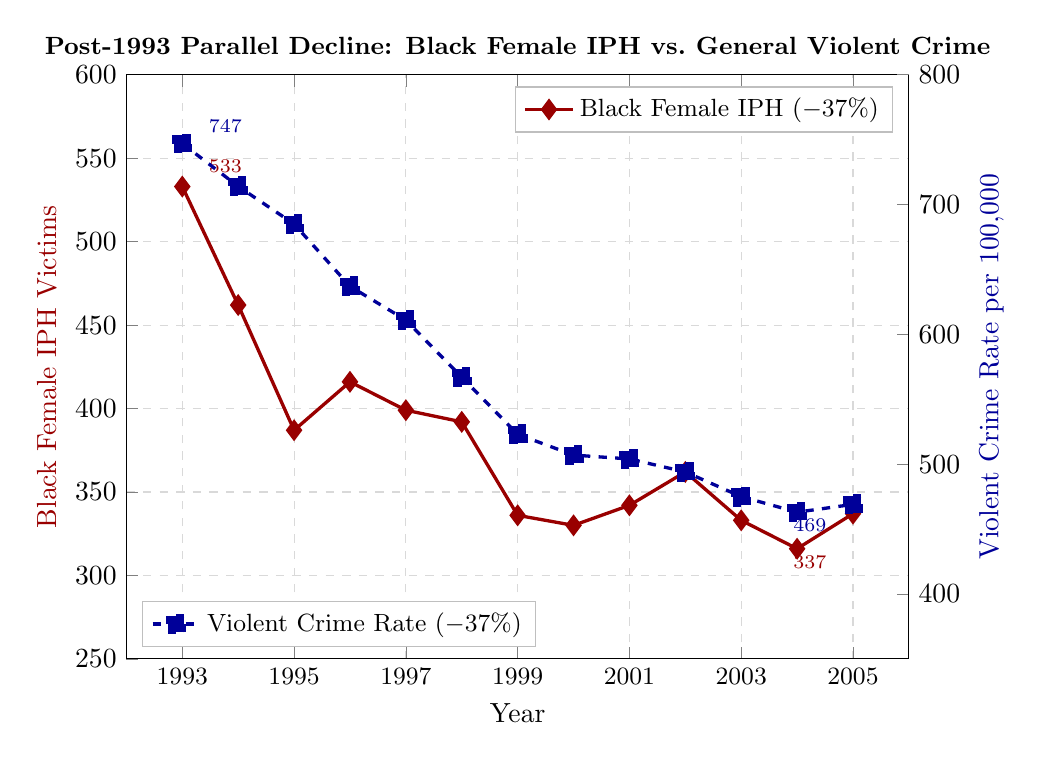
\begin{tikzpicture}
\begin{axis}[
    width=0.95\textwidth,
    height=9cm,
    title={\textbf{Post-1993 Parallel Decline: Black Female IPH vs.\ General Violent Crime}},
    xlabel={Year},
    ylabel={Black Female IPH Victims},
    axis y line*=left,
    xmin=1992, xmax=2006,
    ymin=250, ymax=600,
    xtick={1993,1995,1997,1999,2001,2003,2005},
    xticklabel style={font=\small, /pgf/number format/1000 sep={}},
    grid=major,
    grid style={dashed, gray!30},
    mark size=2.5pt,
    ylabel style={red!60!black},
    legend style={at={(0.98,0.98)}, anchor=north east, font=\small, draw=gray!50},
    every axis title/.style={font=\bfseries\small, at={(0.5,1.05)}},
]
\addplot[very thick, red!60!black, mark=diamond*, mark options={fill=red!60!black, scale=1.2}] coordinates {
    (1993,533) (1994,462) (1995,387) (1996,416) (1997,399)
    (1998,392) (1999,336) (2000,330) (2001,342) (2002,362)
    (2003,333) (2004,316) (2005,337)
};
\addlegendentry{Black Female IPH ($-$37\%)}

\node[font=\scriptsize, red!60!black, anchor=west] at (axis cs:1993.3,545) {533};
\node[font=\scriptsize, red!60!black, anchor=east] at (axis cs:2004.7,308) {337};

\end{axis}
\begin{axis}[
    width=0.95\textwidth,
    height=9cm,
    axis y line*=right,
    axis x line=none,
    ylabel={Violent Crime Rate per 100{,}000},
    xmin=1992, xmax=2006,
    ymin=350, ymax=800,
    ylabel style={blue!60!black},
    mark size=2.5pt,
    legend style={at={(0.02,0.02)}, anchor=south west, font=\small, draw=gray!50},
]
\addplot[very thick, blue!60!black, mark=square*, mark options={fill=blue!60!black, scale=1.2}, dashed] coordinates {
    (1993,747) (1994,714) (1995,685) (1996,637) (1997,611)
    (1998,567) (1999,523) (2000,507) (2001,504) (2002,494)
    (2003,475) (2004,463) (2005,469)
};
\addlegendentry{Violent Crime Rate ($-$37\%)}

\node[font=\scriptsize, blue!60!black, anchor=west] at (axis cs:1993.3,760) {747};
\node[font=\scriptsize, blue!60!black, anchor=east] at (axis cs:2004.7,453) {469};

\end{axis}
\end{tikzpicture}
\caption{\textbf{Parallel Post-1993 Declines.} Black female IPH (left axis, red solid) and the general violent crime rate (right axis, blue dashed) both declined approximately 37\% from 1993 to 2005. The synchronous decline is consistent with the ``detoxified generation'' hypothesis: as the cohort born after the leaded gasoline phase-out ages into the offending window, both public and intimate violence decline in tandem. Sources: FBI SHR \citep{fox2007}; FBI UCR.}
\label{fig:parallel_decline}
\end{figure}

\section{Discussion}

\subsection{Why This Connection Has Not Been Made}

The absence of this analysis from the literature is attributable to disciplinary silos. Environmental epidemiology journals (e.g., \textit{Environmental Health Perspectives}, \textit{Environmental Research}) publish lead-crime studies that operationalize outcomes as aggregate crime. IPV journals (e.g., \textit{Violence Against Women}, \textit{Journal of Interpersonal Violence}) publish domestic violence research using psychosocial and feminist frameworks. These literatures attend different conferences, cite different canonical works, and train different graduate students. The result is a gap that is intellectually obvious once identified but institutionally invisible because no discipline owns both sides of the question.

\subsection{The Underreporting Feedback Loop}

The measured IPH data---which requires a dead body and a police report---captures only the lethal tip of a massive iceberg of nonfatal intimate partner violence. In the specific communities most affected by environmental lead, underreporting of nonfatal IPV was severe due to:
\begin{itemize}[nosep]
    \item Distrust of law enforcement in over-policed communities
    \item Fear of criminalizing Black male partners during the era of mass incarceration
    \item The ``Strong Black Woman'' archetype and community loyalty norms
    \item Lack of culturally competent domestic violence services
    \item Fear of being criminalized as the ``aggressor'' when seeking help \citep{west2022, pmccrossroad2021}
\end{itemize}

The system that created the biological preconditions for intimate partner violence (lead $\rightarrow$ impulse control impairment) simultaneously made it functionally difficult for Black women to report that violence---because reporting meant feeding their partners into the carceral apparatus already designed to consume Black men. The production and the measurement of harm were suppressed by the same structural architecture.

\subsubsection{The Mandatory Arrest Paradox}

The reporting deterrent is not merely anecdotal; it is empirically measurable. Research on mandatory arrest laws---statutes requiring police to make an arrest when responding to a domestic violence call---reveals a paradoxical outcome: states adopting mandatory arrest policies experienced an approximately \textbf{60\% increase in intimate partner homicide} \citep{iyengar2009}. The mechanism is counterintuitive but structurally coherent: the certainty of arrest deters \textit{reporting} rather than \textit{violence}. Victims who know their partner will be arrested upon police contact are less likely to call during early-stage escalation. The suppression of early intervention allows domestic conflicts to escalate unchecked to lethal levels.

This finding directly compounds the lead-IPV hypothesis. In redlined communities during the peak-exposure era, two reporting deterrents operated simultaneously: (1) the generalized distrust of law enforcement in over-policed communities, and (2) the mandatory arrest mechanism that transformed any call for help into an automatic incarceration event. For Black women living with lead-impaired partners whose impulse control was neurologically degraded, the institutional architecture designed to ``protect'' them functioned as a barrier to the early intervention that might have prevented escalation to homicide. The system suppressed the signal (reporting) while amplifying the source (lead-induced aggression).

\subsection{The Bidirectional Cognitive Trap}

An underexplored dimension: lead's effects on executive function---planning, risk assessment, future-oriented decision-making---may have simultaneously degraded women's capacity to recognize danger escalation patterns and execute escape plans. Both partners in lead-exposed communities were cognitively compromised by the same environmental toxin, creating a bidirectional trap that neither partner had the full neurological resources to escape.

\subsection{Implications for the IPV Literature}

If the lead-IPV hypothesis is validated through formal econometric testing, it would require a fundamental expansion of the IPV causal framework. Current models identify risk factors at the individual level (substance abuse, childhood trauma, impulse control deficits) and the structural level (poverty, community violence, systemic racism). Environmental neurotoxicology---the idea that the physical environment in which a community lives can biologically alter the capacity for nonviolent conflict resolution---has never been incorporated as a variable. The spatial precision of lead deposition onto redlined communities means that lead is not a generic environmental stressor but a racially targeted one, produced by identifiable policy decisions with documented racial intent.

\subsection{The Complete Causal Architecture}

Figure~\ref{fig:causal_chain} synthesizes the full argument of this paper into a single causal architecture, tracing the pathway from policy decisions to the invisible epidemic of intimate partner violence.

\begin{figure}[H]
\centering
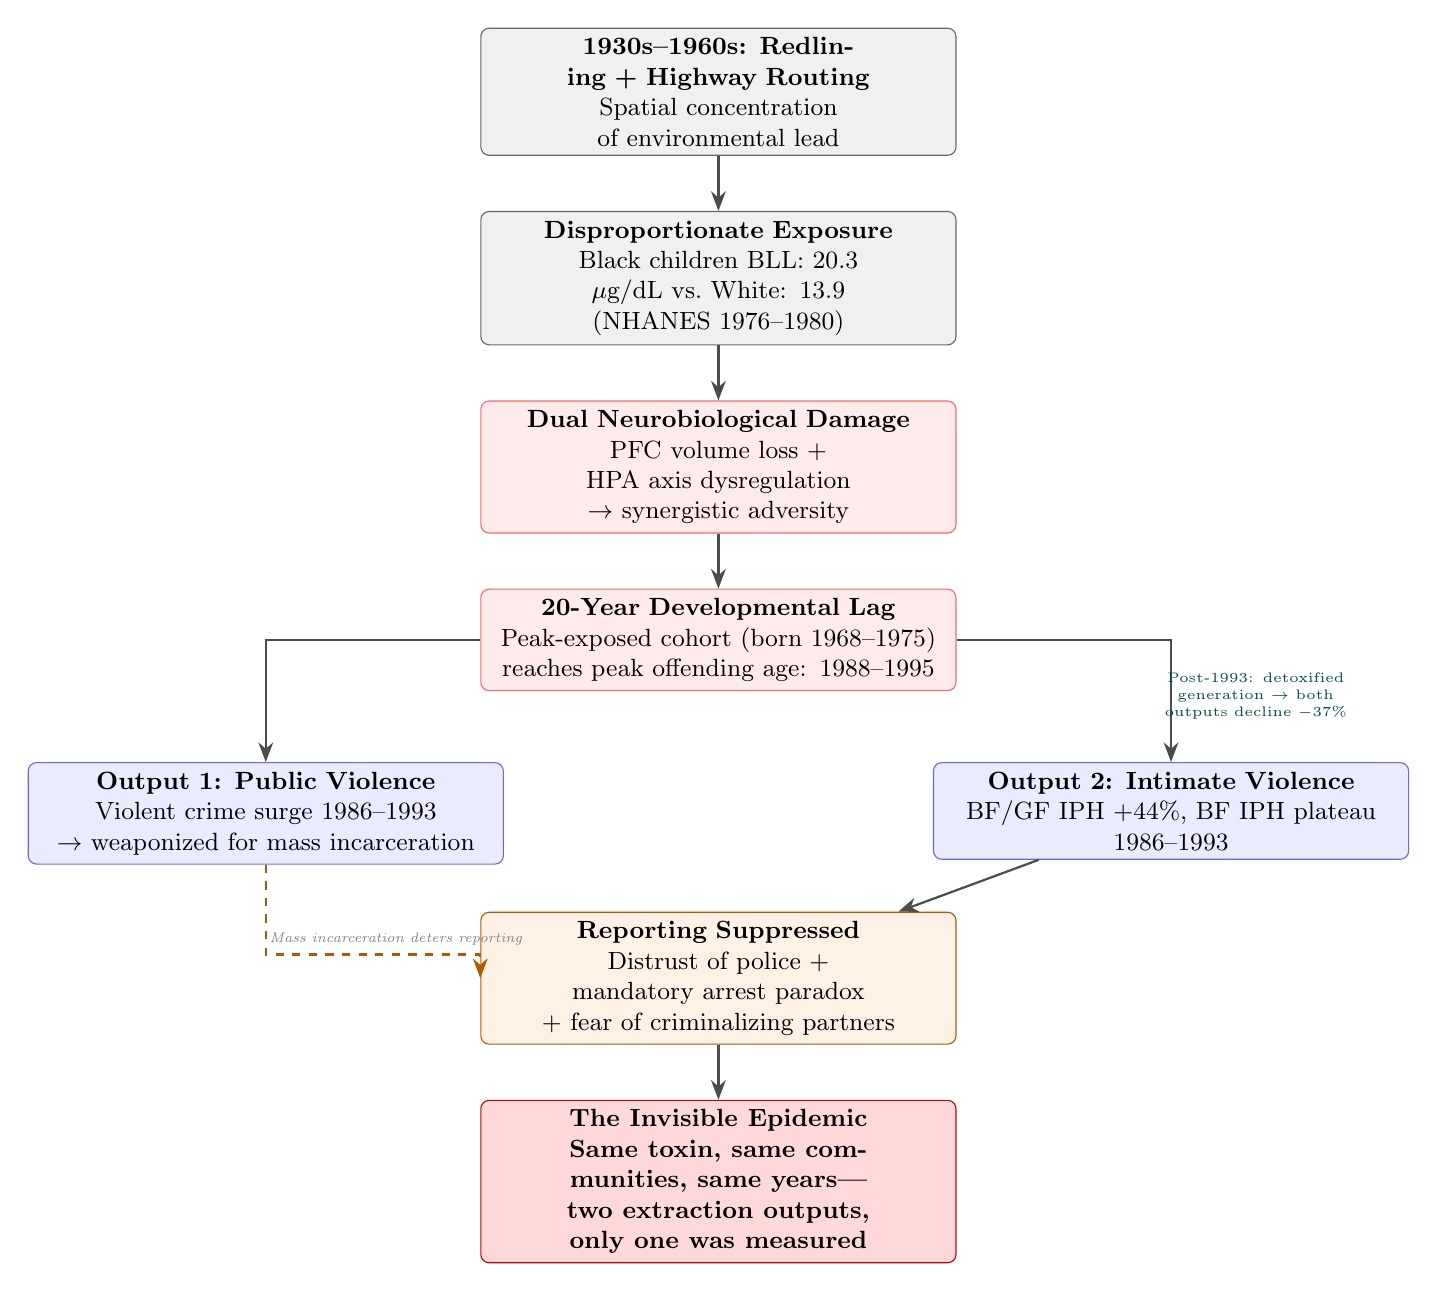
\begin{tikzpicture}[
    node distance=0.7cm,
    every node/.style={font=\small},
    policy/.style={rectangle, draw=black!60, fill=gray!12, text width=5.8cm, align=center, rounded corners=3pt, minimum height=0.85cm},
    bio/.style={rectangle, draw=red!60, fill=red!8, text width=5.8cm, align=center, rounded corners=3pt, minimum height=0.85cm},
    output/.style={rectangle, draw=blue!60, fill=blue!8, text width=5.8cm, align=center, rounded corners=3pt, minimum height=0.85cm},
    suppress/.style={rectangle, draw=orange!70!black, fill=orange!10, text width=5.8cm, align=center, rounded corners=3pt, minimum height=0.85cm},
    final/.style={rectangle, draw=red!80!black, fill=red!15, text width=5.8cm, align=center, rounded corners=3pt, minimum height=0.95cm, font=\small\bfseries},
    arrow/.style={-{Stealth[length=2.5mm]}, thick, black!70},
    label/.style={font=\tiny, black!50, anchor=west},
]

% Policy chain
\node[policy] (redline) {\textbf{1930s--1960s: Redlining + Highway Routing}\\Spatial concentration of environmental lead};
\node[policy, below=of redline] (exposure) {\textbf{Disproportionate Exposure}\\Black children BLL: 20.3 $\mu$g/dL vs.\ White: 13.9\\(NHANES 1976--1980)};
\node[bio, below=of exposure] (damage) {\textbf{Dual Neurobiological Damage}\\PFC volume loss + HPA axis dysregulation\\$\rightarrow$ synergistic adversity};
\node[bio, below=of damage] (lag) {\textbf{20-Year Developmental Lag}\\Peak-exposed cohort (born 1968--1975)\\reaches peak offending age: 1988--1995};

% Dual output
\node[output, below left=0.9cm and -0.3cm of lag] (public) {\textbf{Output 1: Public Violence}\\Violent crime surge 1986--1993\\$\rightarrow$ weaponized for mass incarceration};
\node[output, below right=0.9cm and -0.3cm of lag] (private) {\textbf{Output 2: Intimate Violence}\\BF/GF IPH +44\%, BF IPH plateau\\1986--1993};

% Suppression
\node[suppress, below=2.8cm of lag] (suppress) {\textbf{Reporting Suppressed}\\Distrust of police + mandatory arrest paradox\\+ fear of criminalizing partners};

% Final
\node[final, below=of suppress] (invisible) {\textbf{The Invisible Epidemic}\\Same toxin, same communities, same years---\\two extraction outputs, only one was measured};

% Arrows
\draw[arrow] (redline) -- (exposure);
\draw[arrow] (exposure) -- (damage);
\draw[arrow] (damage) -- (lag);
\draw[arrow] (lag) -| (public);
\draw[arrow] (lag) -| (private);
\draw[arrow] (private) -- (suppress);
\draw[arrow] (suppress) -- (invisible);

% Feedback arrow from public to suppress
\draw[arrow, dashed, orange!70!black] (public.south) |- ([yshift=0.3cm]suppress.west) -- (suppress.west);
\node[label, rotate=0] at ([xshift=-2.8cm, yshift=0.5cm]suppress.west) {\textit{Mass incarceration deters reporting}};

% Post-1993 annotation
\node[font=\tiny, teal!60!black, text width=3cm, align=center, anchor=north] at ([xshift=3.8cm, yshift=-0.3cm]lag.east) {Post-1993: detoxified\\generation $\rightarrow$ both\\outputs decline $-$37\%};

\end{tikzpicture}
\caption{\textbf{The Complete Causal Architecture: From Redlining to the Invisible Epidemic.} Environmental lead, concentrated in redlined communities through deliberate policy, produced two parallel outputs through the same biological mechanism: public violence (weaponized for mass incarceration) and intimate violence (suppressed by the very carceral apparatus the public violence justified). The mass incarceration feedback loop (dashed arrow) further suppressed reporting, ensuring that the gendered harm remained invisible. Both outputs declined in tandem after 1993 as the detoxified generation displaced the lead-damaged cohort.}
\label{fig:causal_chain}
\end{figure}

\section{Proposed Research Agenda}

\subsection{Option 1: Reyes Replication with IPV as Dependent Variable}

Reyes's \citeyearpar{reyes2007} methodology used the state-by-state phase-out of leaded gasoline under the Clean Air Act as a natural experiment. The same approach can be applied:
\begin{itemize}[nosep]
    \item \textbf{Independent variable:} State-level childhood lead exposure (EPA gasoline lead data, CDC blood lead surveys). The CDC archive provides historical de-identified data extracts with county-level specificity, enabling identification of geographic hot spots and construction of lagged exposure variables \citep{cdc_lead_archive}.
    \item \textbf{Dependent variable:} State-level IPH rates from FBI SHR, disaggregated by race and gender. The Easy Access to the FBI's Supplementary Homicide Reports (EZASHR) tool allows researchers to isolate specific victim-offender relationship categories. As of 2019, the IPH subset includes: wife killed by husband (482), husband killed by wife (85), girlfriend killed by boyfriend (505), and boyfriend killed by girlfriend (187)---confirming that the boyfriend/girlfriend category has surpassed spousal IPH as the dominant intimate homicide type in the contemporary period.
    \item \textbf{Lag:} 15--25 years (testing multiple specifications across the developmental window)
    \item \textbf{Prediction:} States that phased out leaded gasoline earlier should show earlier IPH declines
\end{itemize}

\subsubsection{Required Control Variables}

Models must integrate state-level institutional and social policy variables to avoid omitted variable bias, as legal and social structures significantly influence IPV/IPH outcomes independently of lead exposure:
\begin{itemize}[nosep]
    \item \textbf{Mandatory arrest laws:} Statutory adoption dates by state, controlling for the paradoxical 60\% IPH increase documented by \citet{iyengar2009}
    \item \textbf{Firearm access:} State-level prohibitions for DV offenders beyond federal law (IPUMS CDOH)
    \item \textbf{Shelter resources:} DV shelter density and distance metrics. Rural survivors live approximately 3$\times$ farther from resources; 25\% live 40+ miles from the nearest shelter
    \item \textbf{Economic disparity:} Median earnings ratios (male/female) by state and year (IPUMS CDOH)
    \item \textbf{Standard socioeconomic controls:} Poverty rate, unemployment, urbanization, divorce rate
\end{itemize}

\noindent All geographic joins require both state and county FIPS codes. Police-reported data (NIBRS) should be up-adjusted using NCVS reporting rates to account for the ``dark figure'' of domestic violence---the significant gap between reported incidents and actual victimization volume.

\subsection{Option 2: Individual-Level Longitudinal Analysis}

Existing longitudinal cohorts (Cincinnati Lead Study, ELEMENT cohort) have tracked childhood blood lead levels linked to adult behavioral outcomes. As documented in Section~2.1.1, the CLS has confirmed the lead-arrest relationship through 30-year follow-up, and the ELEMENT cohort has identified HPA axis disruption as a second biological pathway. Neither cohort has specifically measured IPV perpetration as an endpoint.

A retrospective analysis adding validated IPV measures (e.g., the Conflict Tactics Scale) to these cohorts would provide individual-level evidence. Methodological precedents from the CLS utilize negative binomial regression with robust standard errors to analyze the frequency of arrests from age 18 to 33 \citep{wright2008}. The same regression framework can be applied with IPV perpetration or victimization as the dependent variable.

\subsubsection{Psychosocial Moderators}

Individual-level models must control for life-course variables to isolate the neurotoxic effect of lead from confounding psychosocial pathways:
\begin{itemize}[nosep]
    \item Childhood exposure to interparental conflict (the critical ``social script'' for intimate aggression)
    \item History of household member imprisonment
    \item Inconsistent or punitive discipline practices
    \item Low parental monitoring during adolescence
    \item Parental substance abuse
\end{itemize}

\noindent These moderators interact with lead-induced neurobiological vulnerability to produce the synergistic adversity model described in Section~2.1.1: a biological inability to inhibit aggressive scripts learned in the home environment.

\subsection{Option 3: The Flint Natural Experiment}

The Flint, Michigan water crisis (2014--present) provides a modern natural experiment. Children exposed to lead-contaminated water will reach peak offending age around 2030--2040. Establishing baseline IPV rates now and monitoring prospectively would test the hypothesis with contemporary data. Additionally, adult lead exposure in Flint may produce shorter-lag effects on impulse control and IPV perpetration.

\subsubsection{Data Assets and Methodological Challenges}

The Michigan Youth Violence Prevention Center (MI-YVPC) maintains geospatial crime data for the Flint area, using Kernel Density Functions to identify violence ``hot spots'' per square mile. Available offense categories include assault offenses (2005--2014), homicide offenses (2005--2014), and gun crimes/crimes with weapons.

A critical methodological challenge must be noted: standalone ``Intimate Partner Violence'' categories are typically absent from police geospatial data libraries, including Flint's. Researchers must use assault offenses as a primary proxy and apply regional correction ratios to estimate the IPV burden. Precedents from the Florida Department of Children and Families estimate that approximately 20\% of homicides are domestic-related, providing a baseline ratio---though this figure likely varies substantially by community demographics and reporting culture.

\subsection{Option 4: Geographic Correlation and Spatial Regression}

Granular spatial regression can link facility-level emissions with localized victimization rates. The methodology involves:
\begin{enumerate}[nosep]
    \item \textbf{Extract TRI data:} Retrieve facility-level data on lead compound releases from the EPA Toxics Release Inventory
    \item \textbf{Apply toxicity weights:} Use the EPA's Risk-Screening Environmental Indicators (RSEI) to multiply mass released (lbs) by the specific toxicity weight for lead
    \item \textbf{Calculate hazard quantity:} The resulting value reflects the inherent capacity of the emission to produce adverse health effects
    \item \textbf{Aggregate by geography:} Map hazard quantities to ZIP codes or census tracts to create localized environmental burden scores
\end{enumerate}

\noindent These burden scores can then be correlated with NCVS IPV rates or police call data, controlling for poverty, segregation, and police presence. The inclusion of legacy lead sources (soil contamination from gasoline exhaust, deteriorating paint, and lead service lines) alongside active TRI emissions captures both historical and ongoing exposure pathways.

\section{Conclusion}

The data presented in this paper do not prove causation. They demonstrate temporal alignment between intimate partner homicide patterns and the predictions of the lead-crime lag model with a precision that demands formal investigation. The boyfriend/girlfriend IPH spike---a 44\% increase during a period when all other IPH categories declined---is particularly difficult to explain through existing IPV frameworks alone. The age-of-peak-risk alignment, the Black female IPH plateau during the lead-predicted window, and the post-1993 parallel decline all point toward an environmental variable that has been systematically excluded from the IPV literature.

If validated, the lead-IPV hypothesis would reveal that the same policy architecture that produced the public violent crime surge of the 1980s--1990s---and that was subsequently weaponized to justify mass incarceration---also produced a parallel, largely invisible epidemic of intimate partner violence within the home. Black women in redlined communities were doubly victimized: first by the environmental racism that poisoned their neighborhoods, and second by living with men whose capacity for nonviolent conflict resolution was neurologically degraded by the same poison.

This is intersectionality operating through a biological channel that no prior analysis has named.

\bibliographystyle{apalike}

\begin{thebibliography}{99}

\bibitem[Aizer and Currie, 2019]{aizer2019}
Aizer, A. and Currie, J. (2019).
\newblock Lead and Juvenile Delinquency: New Evidence from Linked Birth, School, and Juvenile Detention Records.
\newblock \textit{Review of Economics and Statistics}, 101(4):575--587.

\bibitem[CDC, 2021]{cdc_lead_archive}
Centers for Disease Control and Prevention (2021).
\newblock Childhood Blood Lead Surveillance Data.
\newblock CDC National Center for Environmental Health, Lead Poisoning Prevention Program.

\bibitem[Cecil et al., 2008]{cecil2008}
Cecil, K.M., Brubaker, C.J., Adler, C.M., Dietrich, K.N., Altaye, M., Egelhoff, J.C., Wessel, S., Elangovan, I., Hornung, R., Jarvis, K., and Lanphear, B.P. (2008).
\newblock Decreased Brain Volume in Adults with Childhood Lead Exposure.
\newblock \textit{PLoS Medicine}, 5(5):e112.

\bibitem[ELEMENT, 2015]{element2015}
Renzetti, S., Curtin, P., Just, A.C., Bello, G., and Gennings, C. (2015).
\newblock An Overview of the ELEMENT Cohort: Prenatal Lead Exposure, HPA Axis Dysregulation, and Neurobehavioral Outcomes.
\newblock In: \textit{Early Life Exposures in Mexico to ENvironmental Toxicants}. National Institute of Environmental Health Sciences.

\bibitem[Frontiers, 2018]{frontiers2018}
de Souza Lisboa, S.F., Bhatt, S., and Bhatt, S.D. (2018).
\newblock A Hypothesis of the Interaction of the Nitrergic and Serotonergic Systems in Aggressive Behavior Induced by Exposure to Lead.
\newblock \textit{Frontiers in Behavioral Neuroscience}, 12:202.

\bibitem[Fox and Zawitz, 2007]{fox2007}
Fox, J.A. and Zawitz, M.W. (2007).
\newblock \textit{Homicide Trends in the United States}.
\newblock Bureau of Justice Statistics, U.S. Department of Justice.

\bibitem[Harper, 2026]{harper2026}
Harper, E. (2026).
\newblock \textit{Redefining Racism: A Computational Framework for Understanding Systemic Oppression}.
\newblock Manuscript.

\bibitem[Iyengar, 2009]{iyengar2009}
Iyengar, R. (2009).
\newblock Does the Certainty of Arrest Reduce Domestic Violence? Evidence from Mandatory and Recommended Arrest Laws.
\newblock \textit{Journal of Public Economics}, 93(1--2):85--98.

\bibitem[Higney et al., 2022]{higney2022}
Higney, A., Hanley, N., and Moro, M. (2022).
\newblock The Lead-Crime Hypothesis: A Meta-Analysis.
\newblock \textit{Regional Science and Urban Economics}, 97:103826.

\bibitem[NHANES, 2016]{nhanes_bll}
Centers for Disease Control and Prevention.
\newblock National Health and Nutrition Examination Survey (NHANES): Blood Lead Levels in Children Aged 1--5.
\newblock NHANES II (1976--1980), NHANES III (1988--1994), and subsequent cycles through 2015--2016.

\bibitem[Needleman et al., 1979]{needleman1979}
Needleman, H.L., Gunnoe, C., Leviton, A., Reed, R., Peresie, H., Maher, C., and Barrett, P. (1979).
\newblock Deficits in Psychologic and Classroom Performance of Children with Elevated Dentine Lead Levels.
\newblock \textit{New England Journal of Medicine}, 300(13):689--695.

\bibitem[Nevin, 2007]{nevin2007}
Nevin, R. (2007).
\newblock Understanding International Crime Trends: The Legacy of Preschool Lead Exposure.
\newblock \textit{Environmental Research}, 104(3):315--336.

\bibitem[Paulozzi et al., 2001]{paulozzi2001}
Paulozzi, L.J., Saltzman, L.E., Thompson, M.P., and Holmgreen, P. (2001).
\newblock Surveillance for Homicide Among Intimate Partners---United States, 1981--1998.
\newblock \textit{MMWR Surveillance Summaries}, 50(SS03):1--16.

\bibitem[Perkins, 2025]{perkins2025}
Perkins, J. (2025).
\newblock Racism's Impact on Black Intimacy.
\newblock \textit{Journal of Black Sexuality and Relationships}, doi:10.1177/10664807251349846.

\bibitem[PMC Crossroad, 2021]{pmccrossroad2021}
Anyikwa, V.A. and Chiarelli-Helminiak, C.M. (2021).
\newblock Caught in the Crossroad: An Intersectional Examination of African American Women Intimate Partner Violence Survivors' Help Seeking.
\newblock \textit{Journal of Interpersonal Violence}, 36(NP):12003--12027.

\bibitem[PMC Impulse Control, 2023]{pmcimpulse2023}
Elbogen, E.B. et al. (2023).
\newblock Mental and Physical Health, Impulse Control, and Intimate Partner Violence Within a Veteran Sample.
\newblock \textit{Journal of Traumatic Stress}, advance online.

\bibitem[PMC Aggression, 2023]{pmcaggression2023}
Watkins, L.E. et al. (2023).
\newblock Impulsivity and Reactive-Proactive Aggression as Mechanisms of Alcohol-Related Sexual Intimate Partner Violence Perpetration.
\newblock \textit{Psychology of Violence}, 13(5):401--410.

\bibitem[Puzone et al., 2000]{puzone2000}
Puzone, C.A., Saltzman, L.E., Kresnow, M., Thompson, M.P., and Mercy, J.A. (2000).
\newblock National Trends in Intimate Partner Homicide, United States, 1976--1995.
\newblock \textit{Violence Against Women}, 6(4):409--426.

\bibitem[Reyes, 2007]{reyes2007}
Reyes, J.W. (2007).
\newblock Environmental Policy as Social Policy? The Impact of Childhood Lead Exposure on Crime.
\newblock \textit{The B.E. Journal of Economic Analysis \& Policy}, 7(1):Article~51.

\bibitem[Wright et al., 2008]{wright2008}
Wright, J.P., Dietrich, K.N., Ris, M.D., Hornung, R.W., Wessel, S.D., Lanphear, B.P., Ho, M., and Rae, M.N. (2008).
\newblock Association of Prenatal and Childhood Blood Lead Concentrations with Criminal Arrests in Early Adulthood.
\newblock \textit{PLoS Medicine}, 5(5):e101.

\bibitem[West, 2022]{west2022}
West, C.M. (2022).
\newblock The Intersectionality of Intimate Partner Violence in the Black Community.
\newblock In R.\ Geffner et al.\ (Eds.), \textit{Handbook of Interpersonal Violence and Abuse Across the Lifespan}. Springer.

\end{thebibliography}

\end{document}
